\lecture{6}{The Second Law and Entropy}{Qiang Zhu}{scribe-name1,2,3}
%\footnotetext{These notes are partially based on those of Nigel Mansell.}
% **** YOUR NOTES GO HERE:
% Some general latex examples and examples making use of the
% macros follow.  
%**** IN GENERAL, BE BRIEF. LONG SCRIBE NOTES, NO MATTER HOW WELL WRITTEN,
%**** ARE NEVER READ BY ANYBODY.

%\section{Some useful equations} % Don't be this informal in your notes!
%\begin{equation} \label{idealgas} PV = nRT = NkT \end{equation}
%\begin{equation} \label{Avogadro} N = n \times N_A \end{equation}
%\begin{equation} \label{PV-micro} PV = Nm{\overline v_x^2} = NkT\end{equation}
%\begin{equation} \label{eqpartition} U_\text{thermal} = N \cdot f \cdot \frac{1}{2}kT %\end{equation}
%\begin{equation} \label{1stlaw} \Delta{U} = Q + W \end{equation}
%\begin{equation} \label{work3} \Delta W = - P \Delta{V} \end{equation}

\section{Two Interacting Einstein Solids}
In the previous section, we just learned how to count the $\Omega$ for an Einstein solid.
Remember we are trying to understand how heats are transferred, which essentially at least two solids.
Let's call the two solids $A$ and $B$ separately. \\\\
\begin{figure}[h]
\centering
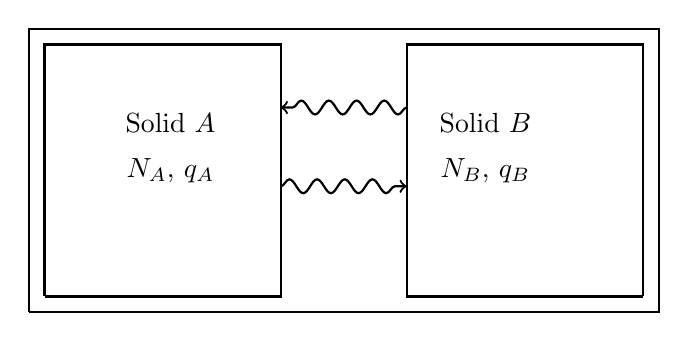
\begin{tikzpicture}[thick]
\draw (0,0.4) -- (8,0.4) -- (8,4) -- (0,4) -- (0,0.4);
\draw (0.2,0.6) -- (3.2,0.6) -- (3.2,3.8) -- (0.2,3.8) -- (0.2,0.6);
\node at (1.8,2.8) {Solid $A$};
\node at (1.8,2.2) {$N_A$, $q_A$};
\draw (7.8,0.6) -- (4.8,0.6) -- (4.8,3.8) -- (7.8,3.8) -- (7.8,0.6);
\node at (5.8,2.8) {Solid $B$};
\node at (5.8,2.2) {$N_B$, $q_B$};
\draw [->,decorate,decoration=snake] (3.2,2) -- (4.8,2);
\draw [->,decorate,decoration=snake] (4.8,3) -- (3.2,3);
\end{tikzpicture}
\caption{Two interacting Einstein solids isolated from the rest of the universe.}
\end{figure}


Assuming that $A$ and $B$ are weakly coupled (just like what we did on ideal gas model),
the individual energies of the solids, $q_A$ and $q_B$ will change slowly.
Under this assumption, the total number of energies $q_\text {total}$ will be simple the sum of $q_A$ and $q_B$.

To make life easier, let's fix $q_\text{total}$, what's the number of multiplicity for any arbitrary $q_A$?
If we just count $A$,
\begin{equation}
 \Omega(A) = \binom{q_A+N_A-1}{q_A},
\end{equation}

In the meantime, we also needs to consider $B$, 
\begin{equation}
 \Omega(B) = \binom{q_B+N_B-1}{q_B},
 q_B = q_ \text {total} - q_A.
\end{equation}

Of course, the total number follows
\begin{equation}
 \Omega(\text {total}) = \Omega(A)\Omega(B).
\end{equation}

{\bf Exercises}\\
Write a table of $q_A$, $\Omega(A)$, $q_B$, $\Omega(B)$, $\Omega$(total), when $q_A$ + $q_B$ = 5, $N_A$=$N_B$=6.

\begin{table}[h]
\centering
\begin{tabular}{|c| c |c |c |c|}\hline
$q(A)$ & $\Omega(A)$ & $q(B)$ & $\Omega(B)$ & $\Omega$(total)\\\hline
    0  &             &        &             &  \\\hline
    1  &             &        &             &  \\\hline
    2  &             &        &             &  \\\hline
    3  &             &        &             &  \\\hline
    4  &             &        &             &  \\\hline
    5  &             &        &             &  \\\hline
\end{tabular}
\end{table}

\section{Stirling Approximation}
To apply these formulas to large systems, we need a trick for evaluating factorials of large numbers. Here is a trick called {\bf Stirling approximation},
\begin{equation}\label{stir}
  N! = N^N e^{-N} \sqrt{2\pi N}
\end{equation}

This can be roughly understood that $N$! is firstly approximated as $N^N$, then averaged by $(N/e)^N$, 
\begin{equation}
  N! = N^N e^{-N} 
\end{equation}

A more elegant way to express $N$! is to use the so called \textbf{Gamma function}. Suppose you start with the integral,
\begin{equation} \int ^\infty _0 e^{-ax} dx = 1/a \end{equation}
and repeat doing differentiation with respect to $a$, you will eventually get
\begin{equation} \int ^\infty _0 x^n e^{-ax} dx = n! a^{-(n+1)} \end{equation}
Starting with this equation, you are able to prove eq \ref{stir}.
From the above, you can get the logarithm as follows
\begin{equation}\label{s1}
      \ln N!  = N \ln N - N - 1/2 \ln (2\pi N) 
\end{equation}

When N is very large, we can safely remove the last term,
\begin{equation}\label{s2}
  \text {ln}N! = N \text {ln}N - N ~~~~~~~~ (\text {when} ~N\rightarrow \infty )
\end{equation}

Alternatively, you can solve it in this way,
\begin{equation}\label{s1}
\begin{split}
      \ln N! & = \ln N + \ln (N-1) + \ln (N-2) + ...    \\
             & \approx \int_0^N \ln x dx \\
             & = N \ln N - N - 1/2 \ln (2\pi N) \\
\end{split}
\end{equation}





\section{Computer Programming}
\begin{enumerate}
\item Write a code to calculate $\Omega$ as a function of $q_A$, when $N_A$=[300, 600, 3000, 6000], $N_B$=[200, 400, 2000, 4000],
and $q$=100, plot them and try to find some tendency when $N$ increases (hint: 4 plots).
\begin{figure}[h]
\centering
\includegraphics[width=12cm]{imgs/Einstein.pdf}
\caption{$\Omega$ as a function of $N$ in two interacting Einstein solids. }
\end{figure}
\item Write a code to calculate the probability of $\Omega(q_A)$, when $N_A$=[300, 3000], $N_B$=[200, 2000],
for $q$=[100, 1000], plot them and try to explain the differences. (hint: 2 plots)

\begin{figure}[h]
\centering
\includegraphics[width=10cm]{imgs/Einstein2.pdf}
\caption{Probability distribution of $\Omega(N)$ in two interacting Einstein solids for different $q$ values. }
\end{figure}

\item Write a code to show the comparison of Stirling approximation in eq.\ref{s1} and \ref{s2}
\begin{figure}[h]
\centering
\includegraphics[width=8cm]{imgs/Stirling.pdf}
\caption{The accuracy of Stirling approximation. }
\end{figure}

\item The Gamma function is defined as 
\begin{equation} \Gamma(n+1) = \int ^\infty _0 x^n e^{-x} dx, \end{equation}
write a code to show the comparison of $\Gamma(n+1)$, $n$!, and $\sqrt{2\pi n}(n/e)^n$ in the range of [0,3.6]
\begin{figure}[h]
\centering
\includegraphics[width=6cm]{imgs/Stirling2.pdf}
\caption{Comparison between the Gamma function and Stirling approximation. }
\end{figure}


\end{enumerate}
